%.-------------------------------------------------------------------------------------------------------------------------------------------------------------
\subsection{UX diagrams}
%.-------------------------------------------------------------------------------------------------------------------------------------------------------------
The mockups of the application were already exposed in the RASD document.
\newline
We present UX diagrams showing the flow all type of users interacts with the system. 
There are repetitions in diagrams to show how mobile application users have lot of common interaction but also web app users have lot of interactions in common.
Every user when application starts up can login or ask to retrieve his/her lost login credentials.
All user can also access statistics and modify their account's data and credentials.
The differences are in some screen available only for specific type of users.
Citizen can create new account and make reports, authorities can take assignments and terminate them, municipality can register  authorities but can also see suggestions , system manager and municipalities can register new municipalities. 
\begin{figure}[h]
\centering
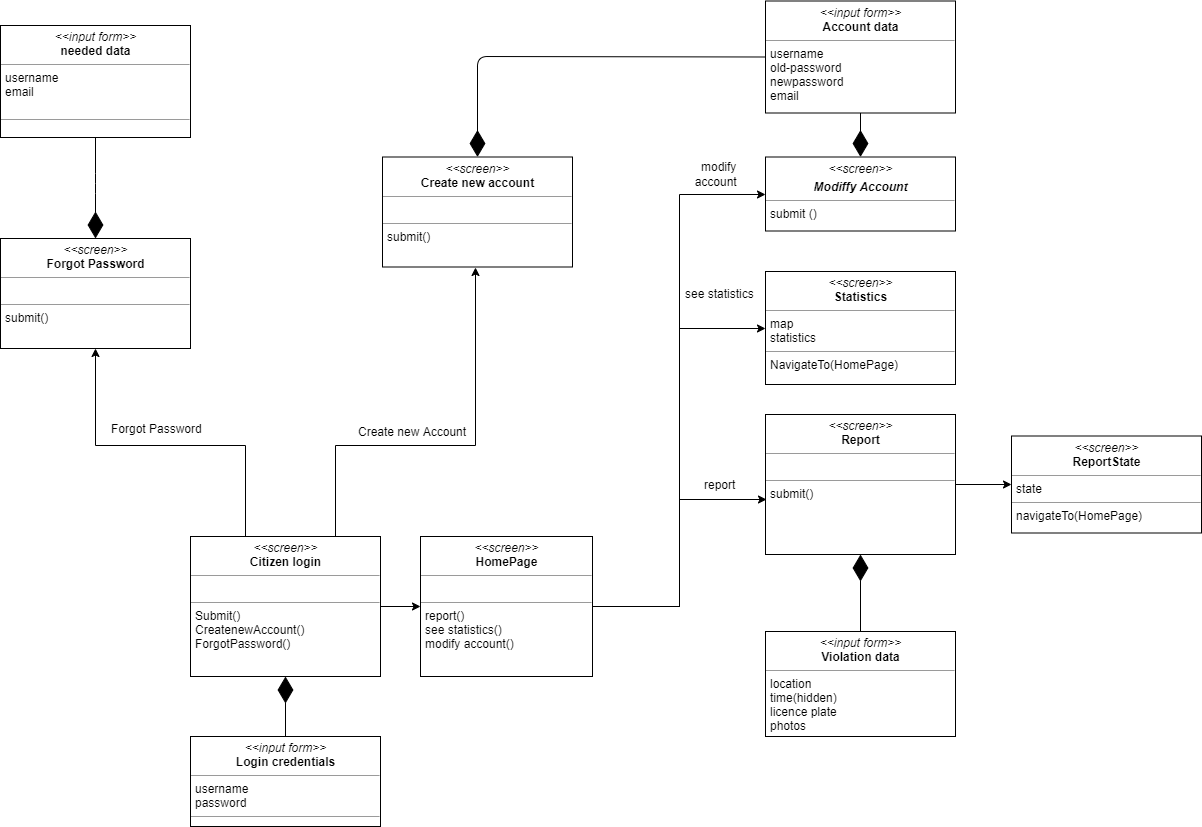
\includegraphics[width=\textwidth]{Images/ux1-correct.png}
\caption{\label{fig:ls}Citizen UX Diagram }
\end{figure}

\begin{figure}[h]
\centering
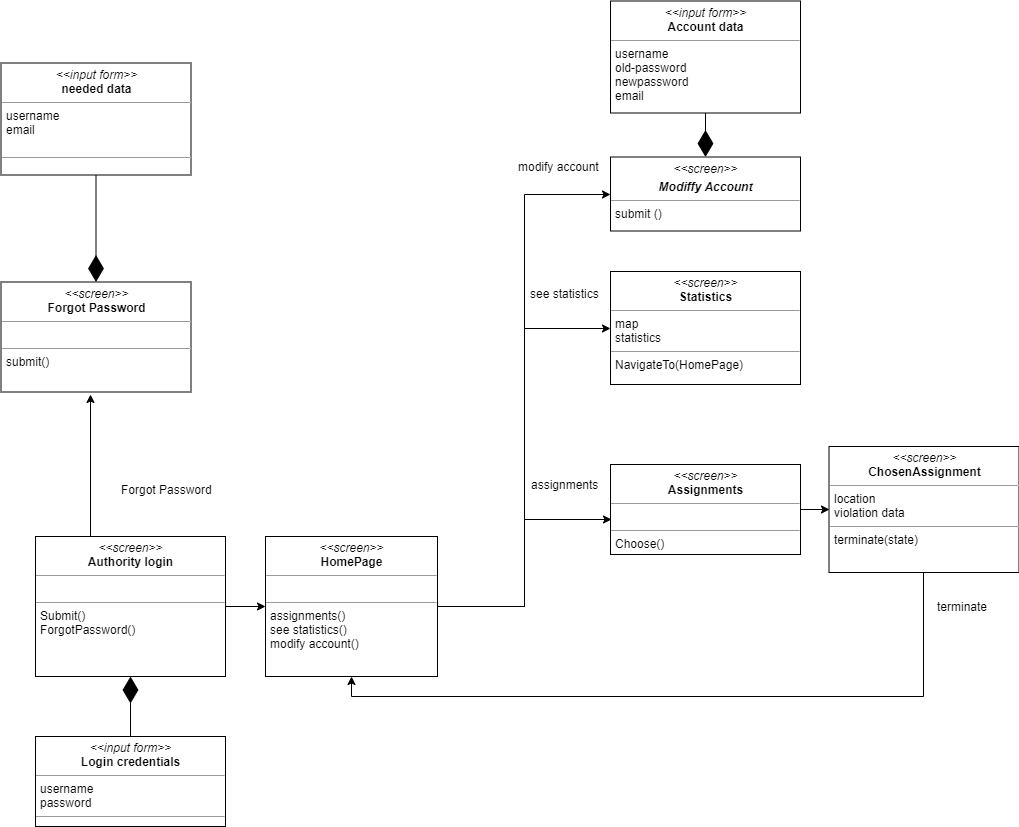
\includegraphics[width=\textwidth]{Images/ux2-correct.png}
\caption{\label{fig:ls}Authority UX Diagram }
\end{figure}
\begin{figure}[h]
\centering
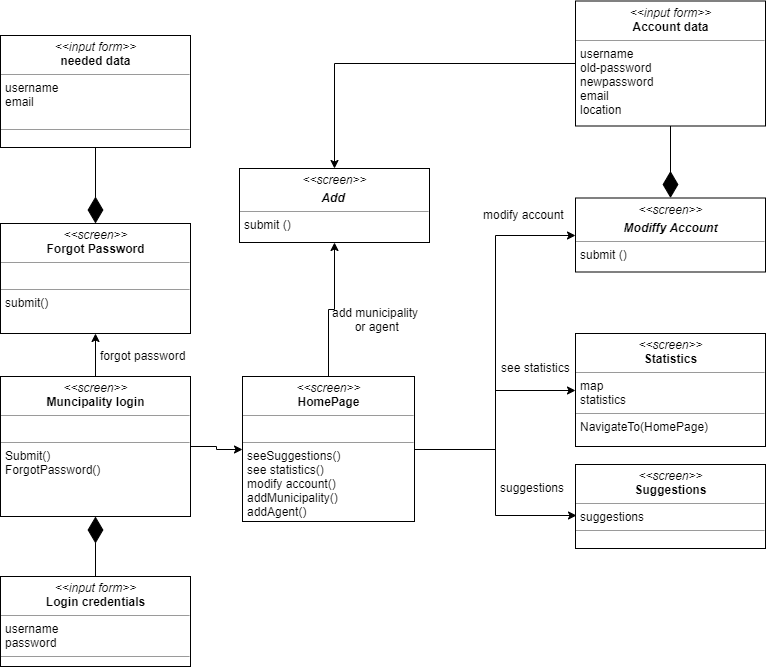
\includegraphics[width=\textwidth]{Images/ux3-correct.png}
\caption{\label{fig:ls}Municipality UX Diagram}
\end{figure}
\begin{figure}[h]
\centering
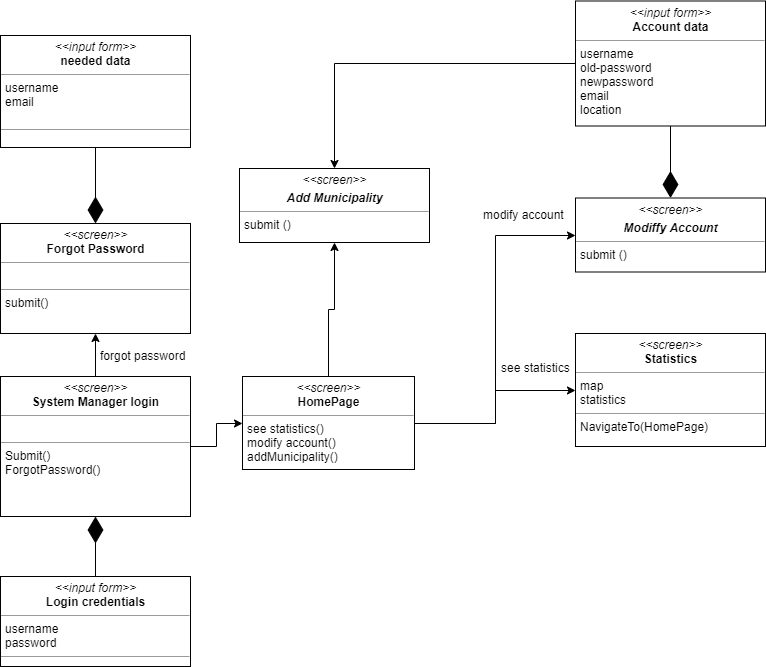
\includegraphics[width=\textwidth]{Images/ux4-correct.png}
\caption{\label{fig:ls}System Manager UX Diagram }
\end{figure}
